\section{Análisis Numérico usando Python}

\begin{enumerate}
    \item Escriba un código en Python que aproxime \( \int_{0}^{1} e^x dx \) usando el método del trapecio con \( n = 10 \).
\end{enumerate}

\begin{figure}[H]
    \centering
    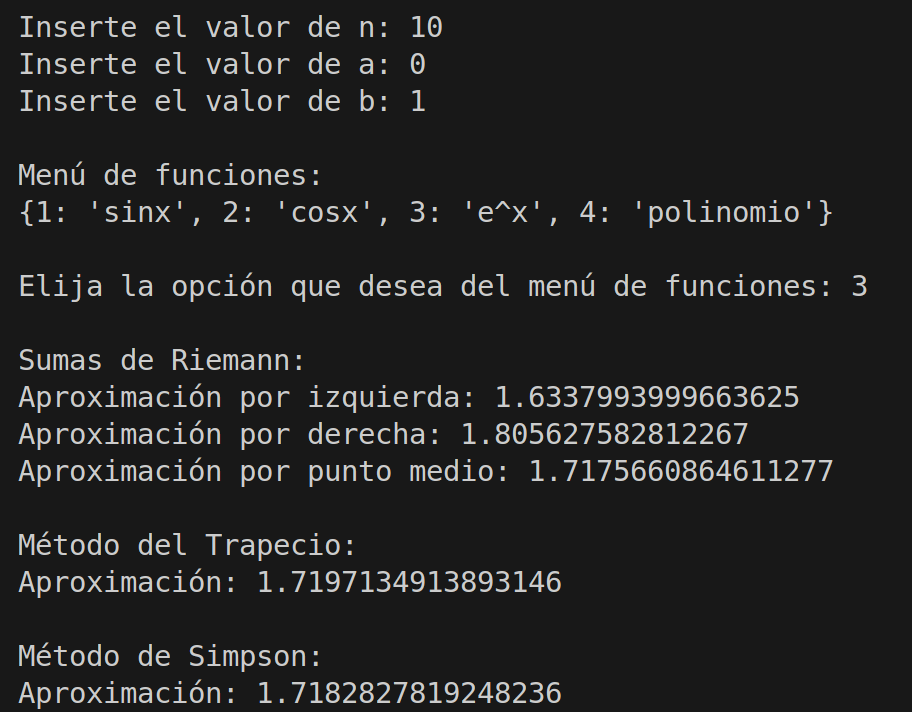
\includegraphics[scale=0.25]{images/python1.png}
    \label{fig:integralEx}
\end{figure}


\begin{enumerate}
    \setcounter{enumi}{1}
    \item Compare la precisión del método del trapecio y el método de Simpson para \( \int_{0}^{\pi} \sin x dx \).
\end{enumerate}

\begin{figure}[H]
    \centering
    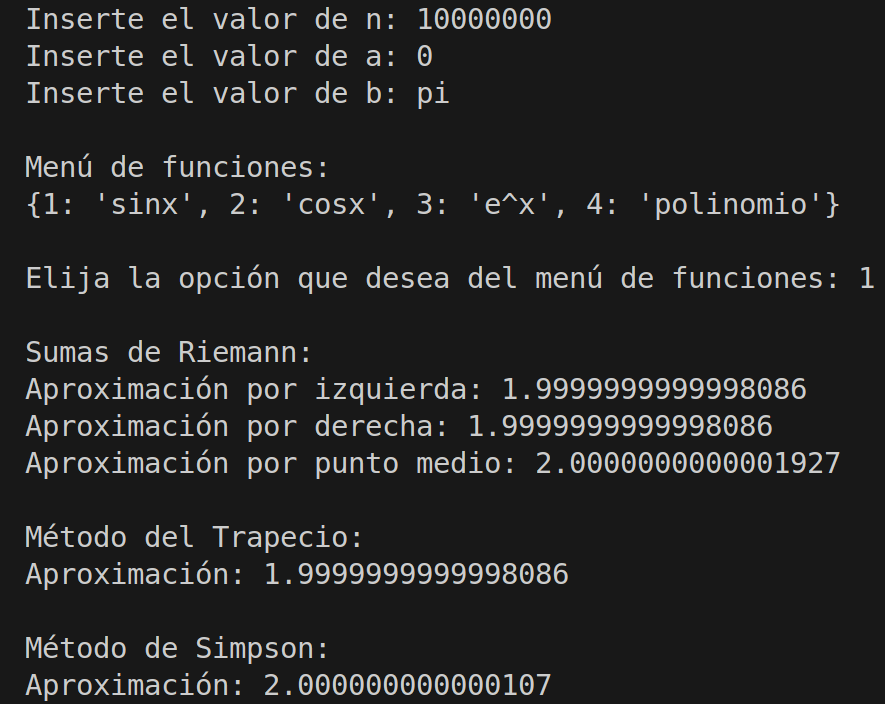
\includegraphics[scale=0.25]{images/python2.png}
    \label{fig:integralSeno}
\end{figure}

Como se ve en la imagen, he escogido un $n$ bastante grande y realmente no hay una diferencia. Usaré un $n = 1$ para ver si hay alguna diferencia.

\begin{figure}[H]
    \centering
    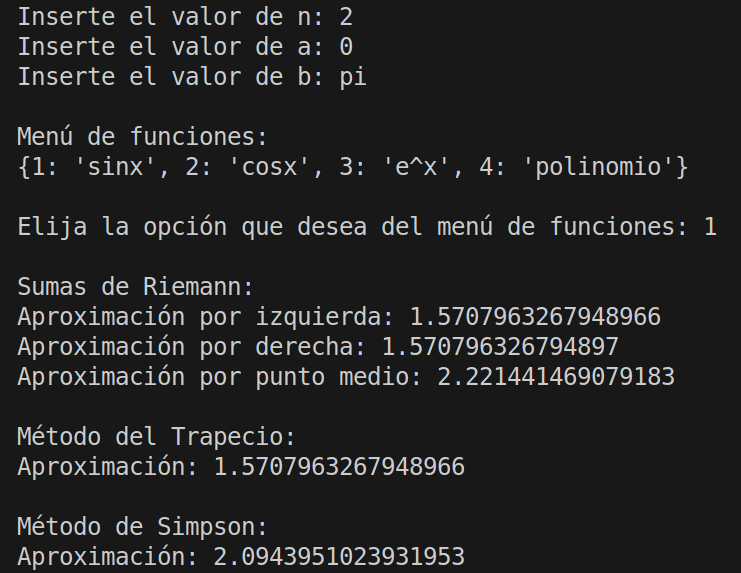
\includegraphics[scale=0.25]{images/python2_1.png}
    \label{fig:integralSeno_Simpson_Trapecio}
\end{figure}

\begin{align*}
    \int_{0}^{\pi} \sin x \,dx 
      &= \left. -\cos x \right|_{0}^{\pi} \\
      &= -\cos \pi - (-\cos 0) \\
      &= -\cos \pi + \cos 0 \\
      &= -(-1) + 1 \\
      &= 2
    \end{align*}

Para \(n = 2\), se han obtenido las siguientes aproximaciones:
\begin{itemize}
    \item \textbf{Método del Trapecio:} \(A_T \approx 1.5708\).
    \item \textbf{Método de Simpson:} \(A_S \approx 2.0947\).
\end{itemize}

El error porcentual se calcula mediante:

\[
\text{Error \%} = \left|\frac{\text{Aproximación} - \text{Valor exacto}}{\text{Valor exacto}}\right| \times 100\%.
\]

\[
\text{Error}_{\text{Trapecio}} = \left|\frac{1.5708 - 2}{2}\right| \times 100\% \approx 21.46\%
\]
\[
\text{Error}_{\text{Simpson}} = \left|\frac{2.0947 - 2}{2}\right| \times 100\% \approx 4.74\%.
\]

El error porcentual para el método de Simpson es significativamente menor que el del método del trapecio, es decir es más preciso.


\begin{enumerate}
    \setcounter{enumi}{2}
    \item Encuentre la integral definida de \( x^3 \) en \([1,2]\).
\end{enumerate}

\begin{figure}[H]
    \centering
    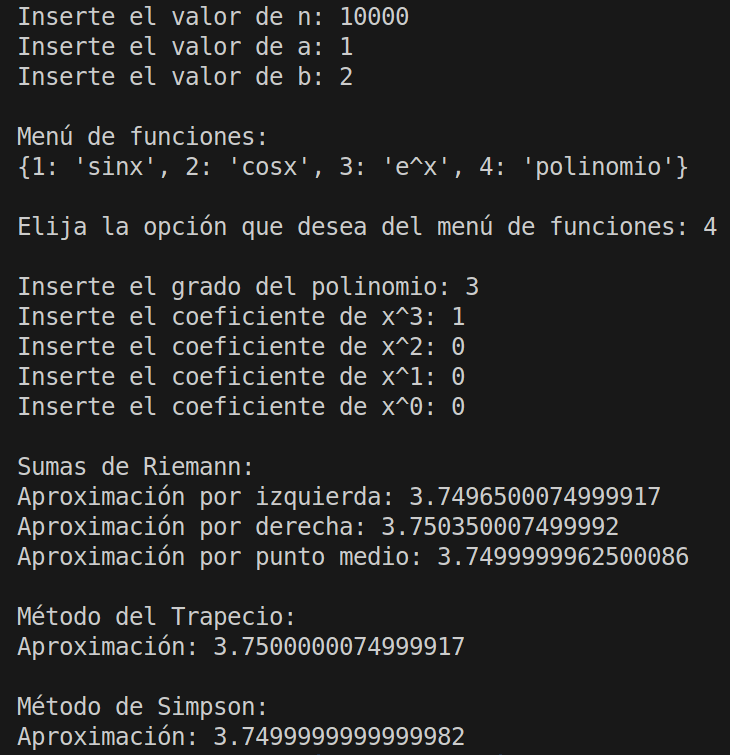
\includegraphics[scale=0.25]{images/python3.png}
    \label{fig:integralCubica}
\end{figure}

\begin{enumerate}
    \setcounter{enumi}{3}
    \item Estime el área bajo la curva \( y = \cos x \) en \([0, \frac{\pi}{2}]\) con el método de Simpson.
\end{enumerate}

\begin{figure}[H]
    \centering
    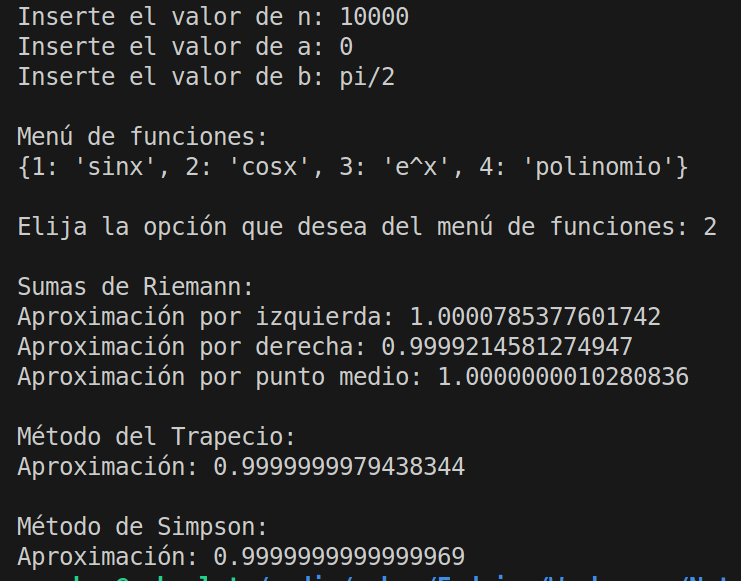
\includegraphics[scale=0.25]{images/python4.png}
    \label{fig:integralCoseno}
\end{figure}